\section{Introduction}

The ``Evaluation of measurement data -- \ac{GUM}'' \cite{JCGMGUM}, or the
``\ac{GUM} bible'', is a foundational international document that provides a
conceptual and mathematical framework for identifying sources of uncertainty,
quantifying them in a consistent way (as standard deviations), combining them
into a single uncertainty figure, and reporting the result and its uncertainty
clearly and comparably across disciplines and countries. Focusing on evaluation
and expression of uncertainty in measurement it is an important component of
the science of measurement and application, known as \gls{metrology} (e.g.,
\cite{JCGMVIM}).

The \ac{GEO} is an international partnership of governments and organizations
acting as a policy and coordination body to promote global sharing and use of
\ac{EO} data, for example to support work on climate, disaster management,
agriculture, water, and ecosystems. The \ac{GEOSS} is the global, distributed
infrastructure that \ac{GEO} is building and coordinating.  Rather than being a
single system, it connects many independent \ac{EO} systems -- such as
satellites, ground networks, and ocean buoys -- from different countries and
agencies, and aims to make them \gls{interoperable}, accessible through common
standards and interfaces, and accompanied by information about data quality and
uncertainty. As such, \ac{GEO} is the partnership, and \ac{GEOSS} is the
``system of systems'' that \ac{GEO} oversees.

To support its mission, \ac{GEOSS} needs a metrological framework. As such, the
2010 endorsement of the \ac{QA4EO} by the \ac{CEOS} (part of \ac{GEOSS}), has
defined guidelines for \ac{EO} applications based on principles adapted from
the metrology community \cite{QA4EO1}. \ac{QA4EO} aims to ensure that \ac{EO}
data are accessible, of known and documented quality, traceable to reference
standards, in particular the \ac{SI}, and suitable for user application
(``fit for purpose''). 

This report aims to further narrow down the scope in applying the \ac{GUM}
principles to \ac{SAR} data. As such, section~\ref{sec:review} provides a
review of the basic and general concepts and terms in \gls{metrology} (the
\ac{VIM}; \cite{JCGMVIM}), the \ac{GUM} \cite{JCGMGUM}, and the \ac{QA4EO}
framework. Section~\ref{sec:level1} and section~\ref{sec:level2} provide the
guidelines to uncertainty estimation for SAR level-1 and level-2 data products,
respectively, as developed in the \ac{ESA} funded \ac{CANVAS} project. Finally,
section~\ref{sec:error_propagation} describes the methods for propagating
errors \ldots, and section~\ref{sec:conclusion} provides the summary and
concluding remarks.

\section{The GUM Principles: A review} \label{sec:review}


%Summary of QA4EO 1 (Executive Summary) and contextualization for QA4SAR



%No need to redefine anything, better to follow same descriptions from:
%Sources: QA4EO, CEOS, SARCALNET, JCGM and its GUM, BIPM, VIM

%\paragraph{CEOS}

\subsection{The International Vocabulary of Metrology (VIM)}

The International Vocabulary of Metrology (\acs{VIM}; \cite{JCGMVIM}) defines
and organizes key concepts in metrology to ensure global consistency in
measurement science. It provides standardized terminology covering quantities,
units, and measuring instruments, with a focus on measurement uncertainty rather
than error.

The document explains critical properties of measuring devices, such as
precision, stability, and sensitivity, and highlights the importance of
traceability and standards for reliability. 

Its applications span various fields, including physics, chemistry, biology,
medicine, and emerging areas like forensic science and food technology.
Harmonization of terms is emphasized to ensure coherence in the various
scientific, engineering, regulatory, and quality assurance fields.

\subsection{Guide to the Expression of Uncertainty in Measurement (GUM)}

The \acf{GUM} establishes general rules for evaluating and expressing
uncertainty in measurement that are intended to be applicable to a broad
spectrum of measurements \cite{JCGMGUM}.  The guide was developed to solve the
challenge of different laboratories and disciplines using different methods and
terminology for uncertainty, which made measurement results difficult to
compare.

The central idea of the \ac{GUM} is to treat all components of uncertainty in
the same mathematical way, regardless of whether they arise from random
variation or systematic effects. Every component is represented by a
probability distribution and a standard uncertainty.  To obtain standard
uncertainties, the \ac{GUM} distinguishes between two kinds of evaluation.
``Type A'' evaluations use statistical analysis of repeated measurements,
whereas ``Type B'' evaluations use all other available information, such as
instrument specifications, calibration certificates, or expert judgment.  The
results of both evaluation types can be converted into standard uncertainties
so they can be used on the same terms.

Measurements are described by a mathematical model that links the quantity
being measured (the \gls{measurand}) to various input, or influence,
quantities. Once standard uncertainties of the influence quantities are
estimated, they are combined -- taking into account any correlations -- using
standard rules for propagating variances. This yields the combined standard
uncertainty of the \gls{measurand}, taken as the estimated standard deviation
associated with the result. An expanded uncertainty is obtained by multiplying
the standard uncertainty by a coverage factor $k$. The purpose of the expanded
uncertainty is  to provide an interval about the result of a measurement that
may be expected to encompass a large fraction of the distribution of values
that could reasonably be attributed to the \gls{measurand}. The value of $k$
and how it was chosen must always be stated.

A key emphasis of the \ac{GUM} is transparency. An uncertainty statement should
clearly describe which inputs were considered, how each uncertainty component
was obtained, what assumptions were made, and how the components were combined.
The document supplements this framework with definitions, statistical
background, guidance on practical evaluation, and worked examples. In doing so,
it provides a common language and method that allow measurement results and
their uncertainties to be understood and compared across borders and domains.


%\paragraph{BIPM}

\subsection{Quality Assurance Framework for Earth Observation (QA4EO)}

% Motivation and specific context of EO

\ac{GEOSS} depends on \gls{interoperable} and quality-assured data to derive
comprehensive information about climate and environment, as well as, e.g.,
food, water and energy security. To achieve \gls{interoperability} across
systems and datasets, common and well-defined data and metadata formats are
needed, but also metrological principles such as \gls{traceability} to \ac{SI},
documented \gls{uncertainty analysis} and \gls{comparison} between different
measurement references must be followed, and are key to the \ac{QA4EO} reports
\cite{QA4EO1}.

% Relation to existing work and projects
Beside \cite{JCGMVIM,JCGMGUM}, \ac{QA4EO} also builds on \ac{EO}-metrology
collaboration in the \ac{EU} \ac{FP7} and Horizon 2020, \ac{ESA} and Copernicus
projects and, in particular, the FIDUCEO project \cite{mittaz19}.

% Principles
As summarized in \cite{QA4EO2}, three basic metrology principles generally
apply to \ac{EO} data:

\begin{enumerate}
  \item {\bf Traceability:}  Metrological traceability is a property of a measurement that relates the measured value to a stated metrological reference through an unbroken chain of calibrations or comparisons. It requires, for each step in the traceability chain, that uncertainties are evaluated and that methodologies are documented.
  \item {\bf Uncertainty Analysis:} Uncertainty analysis is the review of all sources of uncertainty and the propagation of that uncertainty through the traceability chain. It is based on the suite of documents prepared by the \ac{JCGM} and together known as the \ac{GUM}.
  \item {\bf Comparison:} Metrologists validate uncertainty analysis and confirm traceability through comparisons. The Mutual Recognition Arrangement (a formal arrangement to confirm the degree-of-equivalence between \ac{SI} realisations and disseminations in different countries) requires regular, formal international comparisons that are conducted under strict rules.
\end{enumerate}

\noindent The uncertainty analysis, as outlined in the \ac{GUM}, should follow these principles.

% Key Concepts
\ac{ESA} has initially applied the terms \acf{FRM}, \acf{FDR} and \acf{TDP} to
describe metrologically rigorous observations of specific relevance to
space-based observations \cite{QA4EO2}. The terms are increasingly being used
by the broader \ac{EO} community, although they have not yet been formally
endorsed. The terms are defined in \cite{QA4EO2}, as follows:

\begin{itemize}
  \item {\bf Fundamental Data Record (FDR):} An \ac{FDR} is a record, of sufficient duration for its application, of uncertainty-quantified sensor observations calibrated to physical units and located in time and space, together with all ancillary and lower-level instrument data used to calibrate and locate the observations and to estimate uncertainty.
  \item {\bf Thematic Data Product (TDP):} A \ac{TDP} is a record, of sufficient duration for its application, of uncertainty-quantified retrieved values of a geophysical variable, along with all ancillary data used in retrieval and uncertainty estimation.
  \item {\bf Fiducial Reference Measurement (FRM):} An \ac{FRM} is a suite of independent, fully characterised, and traceable (to a community agreed reference, ideally \ac{SI}) measurements of a satellite relevant \gls{measurand}, tailored specifically to address the calibration/validation needs of a class of satellite borne sensors and that follow the guidelines outlined by the \ac{GEO}/\ac{CEOS} \ac{QA4EO}.
\end{itemize}

As highlighted by \cite{QA4EO2}, ``\acp{TDP} provide higher level products that
have been processed from \acp{FDR}, through algorithms which also often combine
information from other \acp{FDR} (e.g., from other satellite sensors) or from
external information (such as reanalysis models and/or certain non-satellite
data), along with such additional information''. Guidelines for assessing
observational systems with respect to \acp{FRM} have been established by
\ac{CEOS} to support the \gls{comparison} principle.


% Approach


\subsection{Metrology}

%Summary of QA4EO 2 (Metrology Theoretical basis)

\subsubsection{Basic concepts}

\paragraph{Metrological observations in EO}

The European Space Agency 

\begin{itemize}
    \item Fundamental Data Record (FDR)
    \item Thematic Data Product (TDP)
    \item \ac{FRM}
\end{itemize}

\paragraph{Uncertainty and error}

%Differences



%Types

\paragraph{Correlation and covariance}
%Correlation
%covariance

\paragraph{The measurement model}


\subsubsection{Principles}

FDRs, TDPs, and \acp{FRM} require a metrological approach. Metrology has three principles:

\begin{enumerate}
    \item Traceability: Documenting the chain of calibrations
    Tractability includes calibration for both the SAR instrument, and the reference instrument (e.g. in situ observations). EO instruments usually require pre-flight, in-orbit and vicarious calibrations, which must be documented. Ancillary and auxiliary data incorporated during the processing of products must also be taken into account along with corrections of any nature (e.g. atmospheric, topographic, etc) and sensitivities to the environment. Similarly, for the reference instrument this principle also includes the deployment calibration and sensitivities to environmental conditions if any. 

    \item Uncertainty Analysis: A systematic approach
      An identification of sources of uncertainties must consider any calibration, instrument changes in orbit and sensitivities to onboard conditions. An analysis of inputs to the measurement model aids to identify those sources. The propagation of those uncertainties through the traceability chain is also part of the analysis. A systematic approach was defined by CEOS and the QA4EO with five steps: Definition of \gls{measurand} and measurement model, creation of a traceability diagram, evaluation of effects, calculation and propagation of uncertainties, and finally documenting. The methodology for this analysis and its five steps is detailed in section 1.4.

    \item Comparison: Validation of uncertainty statements
    EO comparisons are carried out between sensors and between sensors and sub-orbital observations. For metrologists, the purpose of comparisons is to test and validate uncertainty claims. Comparisons are not not performed to estimate uncertainties, but the equivalence ratio. For EO, comparisons are usually performed due to multiple scenes, obervations, and collocations in time. Multiple comparisons require a strong understanding of error correlation structures in the data.  
    
\end{enumerate}


As a graphical summary, Figure 1 summarizes the three metrology principles including the five steps  within Uncertainty Analysis. The flowchart is designed as an iterative process where lessons learned after Comparisons are taken into account for future calibrations.

\begin{figure}
    \centering
    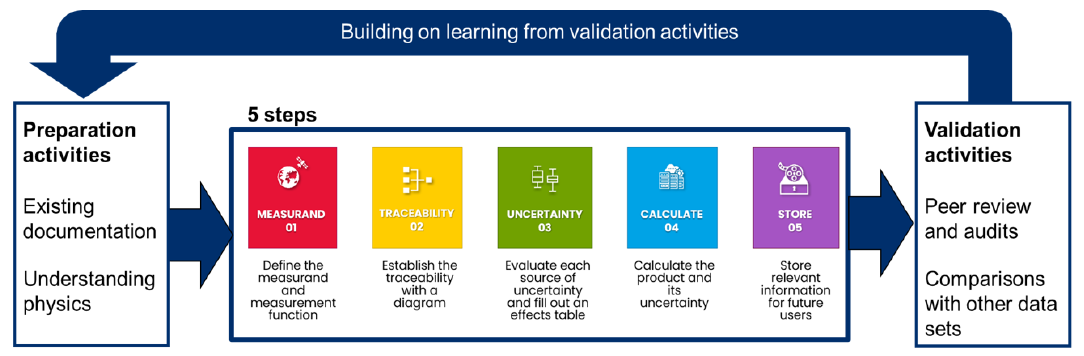
\includegraphics[width=1\linewidth]{figures/Principles.png}
    \caption{An iterative framework for the CEOS Five Steps. Summary of principles including the Uncertainty Analysis five steps.}
    \label{fig:placeholder}
\end{figure}



\subsection{Uncertainty Analysis}

%This is well explained in QA4EO 3 (Process)

There is a consensus in the metrology community about how an uncertainty analysis should be developed. Different EO metrology projects (references) have adapted these stages to emphasize covariance more strongly and have have provided standardized tools for performing some of the analysis.

\subsubsection{Step 1: Measurand and Measurement model definition}

Defining the \gls{measurand} is often the most difficult step, and involves some deep thinking and a challenging conversation between experts. Some experts do not believe that they measure the \gls{measurand}, since the \gls{measurand} may be obtained through a group of algorithms with multiple levels. For these cases, a multi-stage measurement model is considered. The term \gls{measurand} can be applied at different levels of a process and may include both models and observations. The \gls{measurand} can be considered a single point of measurement, e.g. pixel, specific location and/or time, or can represent an area or time period in case of averaged quantities.

The measurement model describes the relationship between the raw input quantities and the \gls{measurand}. This can be an iterative process starting with a more basic model and then including additional quantities to represent the necessary and model approximations. The model should include all the quantities that affects the measurement result. These quantities includes observations and corrections. Well understood effects (i.e. sources of uncertainty) can be directly incorporated as input quantity in the model. Poorly understood effects are usually included in a random variable. It is important to highlight that measurement models are a simplification of a complex reality. A general form of a measurement is describe as:


\[Y=f(X_1,....,X_n; E_1,...., E_n; \Delta_0)\]

Where \(Y\) is the \gls{measurand} as a function of different input quantities from understood effects, \(E\) quantities from poorly understood effects and associated assumptions or approximations.

In some cases the measurement model cannot be described as an analytical model nor a functional relationship. However a description of the different effects can still be produced in order to bring the uncertainty analysis to the next steps. Within EO, many models can be written as univariate or multivariate according to the number of measured values, where one observations can be considered as many observations. As an example, observations of multiple spectral bands or polarizations.


\subsubsection{Step 2: Traceability diagram}

Diagrams can be very useful for \gls{traceability} purposes, identifying sources of uncertainty in input quantities, approximations and assumptions. Four types of diagram have been reported within EO: Uncertainty Tree Diagrams, Processing Diagrams, Metrological \gls{traceability} Diagrams, and Derivation Diagrams.

\paragraph{Uncertainty Tree Diagrams}

Measurement model is put in the centre of the picture and shows the origin of each term of the model. An example from the FIDUCEO project is shown in Figure 2.

\begin{figure}
    \centering
    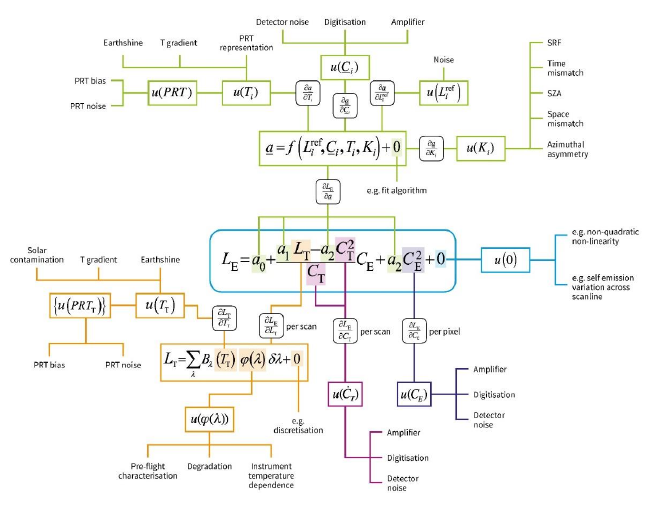
\includegraphics[width=0.7\linewidth]{figures/tree_diagram.png}
    \caption{FIDUCEO uncertainty tree diagram from Mittaz et al 2019}
    \label{fig:placeholder}
\end{figure}

\paragraph{Processing Diagrams}

Representing processing steps or non-analytical processes in a uncertainty tree diagram is difficult. A flow chart is preferable in such cases. Auxiliary information, assumptions and approximations need to be identified for each step of the diagram. Figure 3 shows an example numbering each process. Numbers 1 to 9 belongs to the main processing chain, while other processes for auxiliary and ancillary data are numbered subsequently with the first digit pointing to the linked step from the main chain.

\begin{figure}
    \centering
    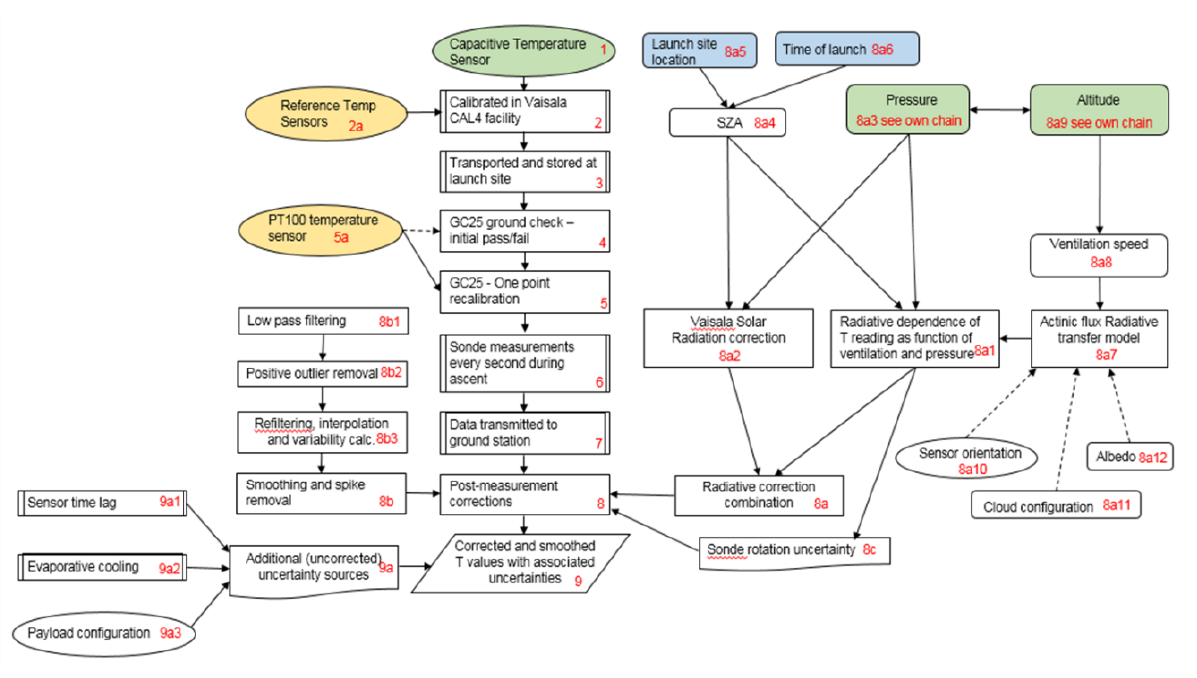
\includegraphics[width=0.7\linewidth]{figures/processing_diagram.png}
    \caption{Example of a processing chain for a RS92 radiosonde temperature measurement}
    \label{fig:placeholder}
\end{figure}

\paragraph{Metrological Traceability Diagrams}

Metrological \gls{traceability} diagrams are a simplified version of processing diagrams, which are suitable for straightforward instruments. The diagram represents the unbroken chain of calibrations. This diagram can also be an auxiliary flow chart for uncertainty tree diagrams. Figure 4 represents a simplified \gls{traceability} chain where the different shapes have different meanings, e.g. processes, auxiliary data, etc.

\begin{figure}
    \centering
    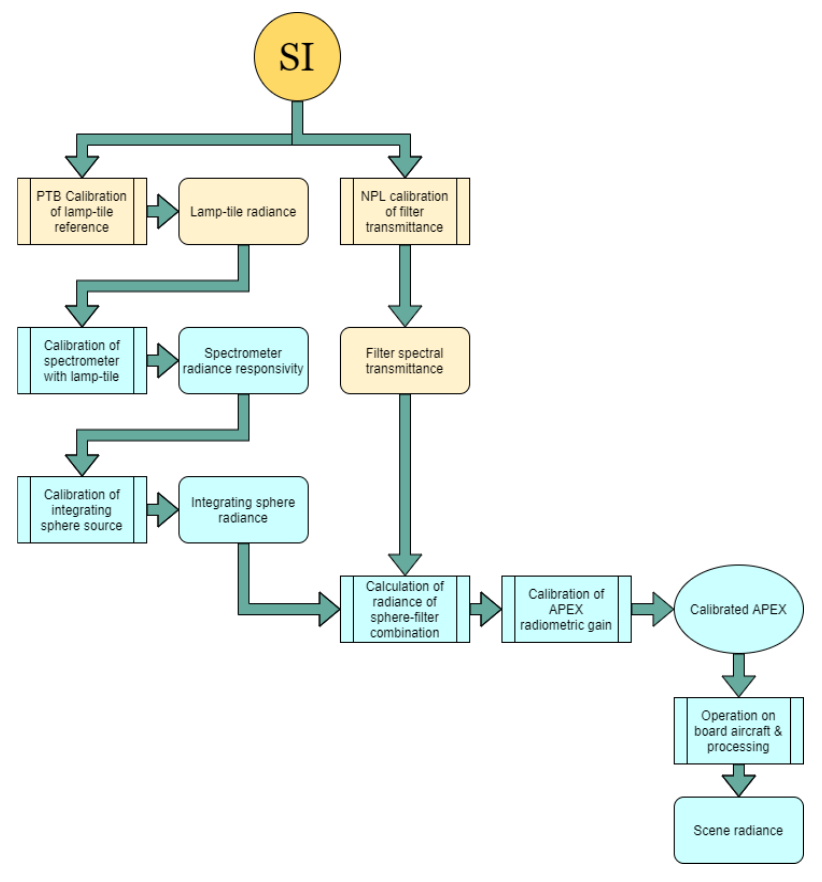
\includegraphics[width=0.7\linewidth]{figures/metrology_diagram.png}
    \caption{Metrological Traceability Diagram for the calibration of the APEX spectrometer carried on the DLR research aircraft.}
    \label{fig:placeholder}
\end{figure}

\paragraph{Derivation Diagrams}

Derivation diagrams are similar to uncertainty tree diagrams in the sense that equations are also provided. However, derivation diagrams are focused on the assumptions within the measurement model. Therefore, derivation diagrams can be described as a uncertainty tree diagram where assumptions and approximations are extensively detailed instead of being represented by a negligible value.

\begin{figure}
    \centering
    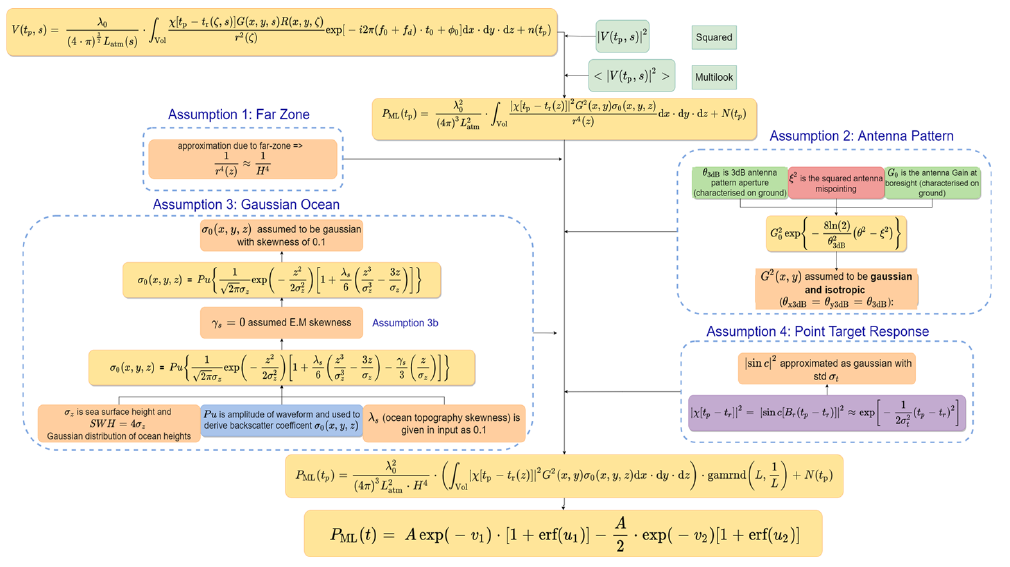
\includegraphics[width=0.7\linewidth]{figures/derivation_diagram.png}
    \caption{Part of the derivation diagram for sea level rise where assumptions are detailed}
    \label{fig:placeholder}
\end{figure}

Although four diagram types are here described, a new, different diagram can be design in order to draw a picture of our system for \gls{traceability} purposes. Different type of diagrams can also be combined.

\subsubsection{Step 3: Evaluation of each source of uncertainty}

After Steps 1 and 2, sources of uncertainty (i.e. effects), assumptions, approximations and corrections  during the observational process have been identified. Then, uncertainties can be propagated though the measurement model, multi-stage or single-stage, until the \gls{measurand}. Before uncertainty propagation some description is necessary for each effect. Hence, the use of an "effect table" is convenient, which provides:

\begin{itemize}
    \item Unique identifier of the effect.
    \item The measurement model term affected by the effect.
    \item Magnitude of the uncertainty.
    \item Existent error correlations, when applicable.
    \item The form of the error correlation for each dimension of interest.
    \item A maturity indicator.
    \item The probability density function (PDF) and/or sensitivity coefficient.
\end{itemize}

Error correlations must also be described for both, correlations between input quantities and between terms within the measurement model. The error correlation structure of each effect must also be determined for each dimension of interest. Dimensions for which different observations will be combined or compared at later processing level.

The maturity of an uncertainty estimate is a qualitative concept. The highest maturity is achieved when two conditions are met: the effect has been evaluated robustly, i.e. properly modeled or repeatedly, and validated by comparison to independent data sets. If only one of the conditions applies, then maturity is moderate. In a low maturity none of the conditions have been met. Instead, expert judgment has been used to estimate the uncertainty magnitude. Table 1 summarizes the requirements of the evaluation of effects into a effects table. An extensive guideline for filling the table is available at QA4EO 3 Appendix B!!!!!! 


\begin{table}[ht]
\centering
\begin{tabular}{|l|l|l|}
\hline
\multicolumn{3}{|c|}{\textbf{EFFECTS TABLE}} \\ \hline
\textbf{Name of effect} & Effect name 1.1 & Effect name 1.2 \\ \hline
\textbf{Effect identifier} & 1.1 & 1.2 \\ \hline
\textbf{Affected term in measurement function} &  &  \\ \hline
\textbf{Maturity of analysis} &  &  \\ \hline
Maturity of uncertainty estimate &  &  \\ \hline
Maturity of correlation scale estimate &  &  \\ \hline
For low maturity, is effect negligible? &  &  \\ \hline
\textbf{Correlation type and form} &  &  \\ \hline
Within dimension 1 &  &  \\ \hline
Within dimension 2 &  &  \\ \hline
Within dimension 3 &  &  \\ \hline
Within dimension 4 &  &  \\ \hline
\textbf{Correlation scale} &  &  \\ \hline
Within dimension 1 &  &  \\ \hline
Within dimension 2 &  &  \\ \hline
Within dimension 3 &  &  \\ \hline
Within dimension 4 &  &  \\ \hline
\textbf{Uncertainty} &  &  \\ \hline
PDF shape &  &  \\ \hline
units &  &  \\ \hline
magnitude &  &  \\ \hline
\textbf{Sensitivity coefficient} &  &  \\ \hline
\end{tabular}

\caption{Example of blank effects table.}
\label{tab:descriptor}
\end{table}

\subsubsection{Step 4: Calculate \ac{FRM}/FDR/TDP associated uncertainties}

A robust uncertainty analysis should highlight where the model can be improved. So, a correction for an effect can be proposed. It is important to identify how large the uncertainty associated is and how it propagates to the \gls{measurand}. The propagation can be undertaken by the Monte Carlo (MC) method, with PDFs of each effect, or by the Law of Propagation of Uncertainties (LPU), with sensitivity coefficient and error covariance matrix for each effect. Propagation is further described in section 1.5.

\subsubsection{Step 5: Documenting}

There are three types of environmental dataset with different requirements when providing uncertainties. 

\begin{enumerate}
    \item Operational data. For near-real time applications timeliness and consistency are extremely important. Uncertainties are often less critical and usually indicated as noise. It may contain quality flags, but covariance information is rarely calculated.
    \item Research data. A combination of near-real time and historical data. Ideally, uncertainty and covariance should be provided, but in simplified format, since the data is provided for applications at higher level.
    \item Long term data preservation. This is the data for future scientists. It should include all the associated metadata and documentation in order to reproduce results and undertake future reanalysis.
\end{enumerate}

\subsection{Uncertainty Propagation}

As mentioned in previous sections, there are two methodologies to propagate uncertainties through the measurement model until the measureand. The first method is the Law of Propagation of Uncertainties (LPU) relies on the error covariance matrices and sensitivity coefficient produced for each output quantity. The second method is the Monte Carlo (MC) method relies on the probability distribution function of each source of uncertainty or, in a compact way, the output quantities. This section details how to apply these methods during the uncertainty analysis.

\subsubsection{Law of Propagation of Uncertainties method}

This method is based on a locally linear approximation to combine uncertainties using the expresion:


\[u^2(y) = \sum_{i=1}^N c_i^2 u^2(x_i) + 2 \sum_{i=1}^{N-1} \sum_{j=i+1}^N c_i c_j u(x_i, x_j)\]

Where \(u^2(y)\) is the combined uncertainty associated with the measured value \(y\). \(u(x_i)\) is the uncertainty associated with the input quantity \(x_i\). \(u(x_i, x_j)\) is the covariance between \(x_i\) and \(x_j\). \(c_i=\delta y/ \delta x_i \) is the sensitivity coefficient, i.e. the relationship between an uncertainty associated to an input quantity and the uncertainty associated to the measured quantity. \(N\) represents the number of input quantities. In this equation the first term, \(\sum_{i=1}^N c_i^2 u^2(x_i)\) is fully independent, while the second term \(2 \sum_{i=1}^{N-1} \sum_{j=i+1}^N c_i c_j u(x_i, x_j)\) stands for the error correlation.

The expression can also be written in matrix form as:


\[u²(y)=cS(x)c^T\]

where \(c=[\delta y/\delta x_1, ..., \delta y/\delta x_N]\) is a row vector of sensitivity coefficients and \(S(x)\) is the error covariance matrix for the input quantities with diagonals \(u²(x_i)\) and off-diagonals \(u(x_i, x_j)\)

\subsubsection{MonteCarlo method}



